\subsection{Auckland}

Comencemos por describir la ruta generada(Ver mapa que todavía no está). Se han realizado 22 saltos hasta alcanzar el destino solicitado, de los cuales en el $72 \% $ de los mismos aproximadamente, hemos obtenido respuestas del tipo $TIME\_EXCEEDED$, determinando, así que el largo de nuestra ruta es de 16 saltos, y que del resto de los valores del $TTL$ no hemos obtenido respuesta alguna. Como también se puede ver en el (mapa que no está), durante el trayecto se realizaron 3 saltos intercontinentales, en los ttls 6, 10 Y 19. Por otro lado, el método de Cimbala nos ha detectado todo número positivo como outlier en primera instancia y al sacar los 0s nos devolvió como outliers los ttls 6, 10, 15, 16, 19, 22.


Al realizar el experimento, se logró llegar al destino en el ttl 22. De estos, 6 no respondieron. Los ttls que Cimbala reconoció como intercontinentales fueron 6, 10, 15, 16, 19, 22.

\begin{figure}[!htbp]
  \centering
    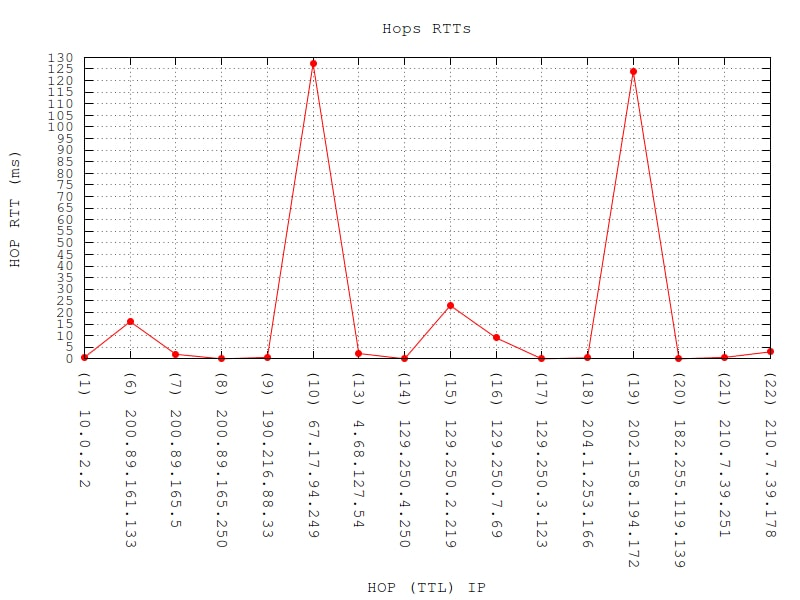
\includegraphics[scale=0.6]{imagenes/auckland-graficos/traceroute-auckland.jpg}
  \caption{auckland- RTT hops}
  \label{fig:7}
\end{figure}

En la figura \ref{fig:7} se puede observar como el ttl 10 y 19 tienen un rtt claramente distinguido del resto.

\begin{figure}[!htbp]
  \centering
    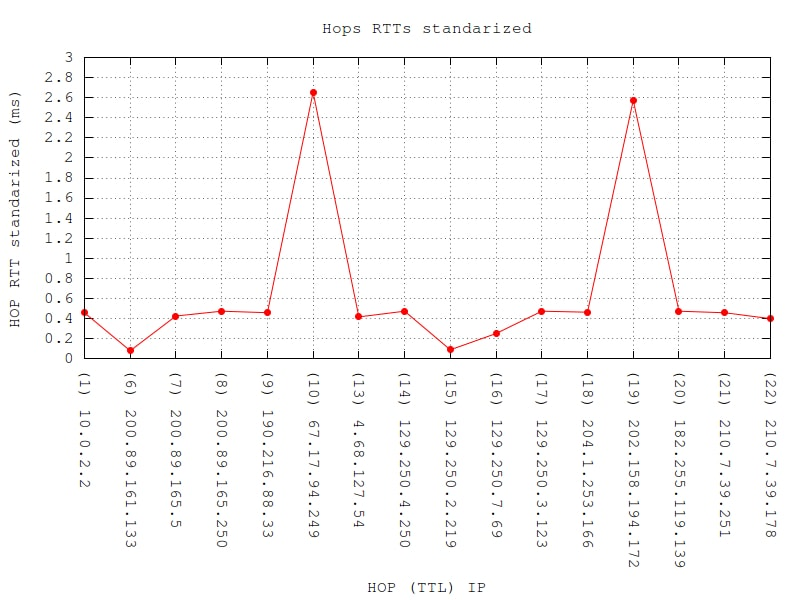
\includegraphics[scale=0.6]{imagenes/auckland-graficos/traceroute-auckland-standarized.jpg}
  \caption{auckland- RTT hops standarized}
  \label{fig:8}
\end{figure}

En la figura \ref{fig:8} se puede observar una situacion similar a la de la figura \ref{fig:7}.


